
%(BEGIN_QUESTION)
% Copyright 2010, Tony R. Kuphaldt, released under the Creative Commons Attribution License (v 1.0)
% This means you may do almost anything with this work of mine, so long as you give me proper credit

Suppose a guided-wave radar transmitter is used to measure the ullage of vessel where the liquid has a relative permittivity of 37 and the vapor has a relative permittivity of 1.2 (at atmospheric pressure and standard temperature):

$$\includegraphics[width=15.5cm]{i04623x01.eps}$$

First, calculate the echo time for an ullage of 1.5 meters (as shown):

\vskip 10pt

$t$ = \underbar{\hskip 50pt}

\vskip 20pt

Next, calculate the echo time assuming the pressure of the vapor increases from 1 atmosphere to 3 atmospheres.

\vskip 10pt

$t$ = \underbar{\hskip 50pt}

\underbar{file i04623}
%(END_QUESTION)





%(BEGIN_ANSWER)

$t$ (at 1 atm) = 10.96 nanoseconds

\vskip 10pt

$t$ (at 3 atm) = 12.66 nanoseconds

%(END_ANSWER)





%(BEGIN_NOTES)


%INDEX% Measurement, level: radar

%(END_NOTES)

